\documentclass[journal,12pt,twocolumn]{IEEEtran}

\usepackage{enumitem}
\usepackage{amsmath}
\usepackage{amssymb}
\usepackage{graphicx}

\title{Assignment 1 \\ \Large AI1110: Probability and Random Variables \\ \large Indian Institute of Technology Hyderabad}
\author{Pranav B \\ \normalsize AI21BTECH11023 \\ \vspace*{20pt} \normalsize  10 April 2022 \\ \vspace*{20pt} \Large ICSE 2019 Grade 10}


\begin{document}
	% The title
	\maketitle
	
	% The question
	\textbf{Question 6(c)} 
	A hemispherical and a conical hole is scooped out of a solid wooden cylinder. Find the volume of the remaining solid where the measurements are as follows:\\
	The height of the solid cylinder is 7 cm ,radius of each of hemisphere,cone and cylinder is 3 cm. Height of cone is 3 cm.\\
	Give your answer correct to the nearest whole number. Take $\pi$=$\frac{22}{7}$\\
	% The solution
	\textbf{Solution.}
	The various parameters involved in this question are listed in Table\\ \begin{table}[h]
\caption{Variables used}
\begin{tabular}{|c |c|c|}
\hline 
\textbf{Parameter} & \textbf{Symbol} & \textbf{Value/Formula}\\
\hline
Radius of cylinder(same as cone and hemisphere) & R & 3 cm\\
\hline
Height of cone removed & h & 3 cm\\
\hline
Height of cylinder & H & 7 cm\\
\hline
Volume of cylinder & V$_1$ & $\pi R^2 H$\\
\hline
Volume of cone  & V$_2$ & $\frac{1}{3} \pi R^2 h$\\
\hline
Volume of hemisphere & V$_3$ & $\frac{2}{3} \pi R^3$\\
\hline
\end{tabular}
\end{table}
\\
According to question Hemisphere, Cone are removed from Cylinder\\
\begin{align}
\therefore \text{remaining volume} = V_1-V_2-V_3
\nonumber
\\
=\pi R^2 H - \frac{1}{3} \pi R^2 h - \frac{2}{3} \pi R^3
\nonumber
\\
\text{Substituting the values above  we get,}
\nonumber
\\
\approx113.142 cm^3
\nonumber
\end{align}
\begin{figure}[ht!]
\begin{flushright}
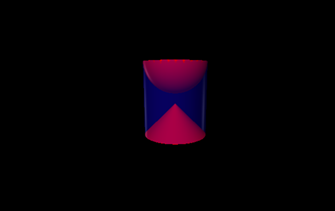
\includegraphics[width=0.38 \textwidth]{Picture1.png}
\end{flushright}
\end{figure}		
\end{document}